\documentclass[dvipdfmx]{beamer}

\usepackage{graphics}
\usepackage{amsmath}
\usepackage{amssymb}
\usepackage{ascmac}
\usepackage{txfonts}
\usepackage{bm}
\usepackage{docmute}
\usepackage{tikz}
\usetikzlibrary{calc}
\usetikzlibrary{intersections}

\usetheme{Madrid}
\usefonttheme{professionalfonts}


\title{質問の答え}
\author{近藤 綜太}

\begin{document}
	\maketitle
	\begin{frame}{問題1}
		以下の4式を計算せよ.
		\begin{gather}
			\left(
				\frac{1}{3}x + \frac{1}{2}y + \frac{1}{6}
			\right)
			\left(
				\frac{1}{3}x - \frac{1}{2}y - \frac{1}{6}
			\right)\\ \nonumber \\
			\left(
				\frac{3}{4}x + \frac{1}{3}y - 2
			\right)
			\left(
				\frac{3}{4}x - \frac{1}{3}y + 2
			\right)\\ \nonumber\\
			\left(
				4x - \frac{1}{2}y
			\right)^2 + 
			\left(
				x + \frac{3}{2}y
			\right)^2\\ \nonumber\\
			\left(
				x + \frac{2}{3}y
			\right)
			\left(
				x - \frac{2}{3}y
			\right)
			+ \frac{1}{3}(2x + y)^2
		\end{gather}
	\end{frame}

	\begin{frame}{公式}
		今日使う公式
		\begin{itemize}
			\item 二乗公式
			\item 和と差の積
		\end{itemize}
		\begin{gather*}
			(a+b)^2 = a^2+ 2ab +b^2\\
			(a-b)^2 = a^2- 2ab +b^2\\
			(a+b)(a-b) = a^2-b^2
		\end{gather*}
	うまく $a, b$に式を当てはめる.
	\end{frame}

	\begin{frame}{解答1-1}
		\begin{align*}
			\left(
				\frac{1}{3}x + \frac{1}{2}y + \frac{1}{6}
			\right)
			\left(
				\frac{1}{3}x - \frac{1}{2}y - \frac{1}{6}
			\right)
			&= \left\{ \frac{1}{3}x 
				+ \left( \frac{1}{2}y + \frac{1}{6}\right)
			\right\}
			\left\{ \frac{1}{3}x 
				- \left( \frac{1}{2}y + \frac{1}{6}\right)
			\right\}\\
			&=\left( \frac{1}{3}x\right)^2 - \left( \frac{1}{2}y - \frac{1}{6}\right)^2\\
			&= \frac{1}{9}x^2  
			-\frac{1}{4}y^2
			+ \frac{1}{6}y
			- \frac{1}{36}
		\end{align*}

		カッコの中に共通点 $ \frac{1}{2}y + \frac{1}{6}$を見つけることが
		できたら,それをまとめて和と差の積の計算にする.
		見つけたあとに別の文字に置き換えてもよい.
	\end{frame}

	\begin{frame}{解答1-2}
		さっきと同じ.共通点を見つけることができたら和と差の積にして計算.
		\begin{align*}
			\left(
				\frac{3}{4}x + \frac{1}{3}y - 2
			\right)
			\left(
				\frac{3}{4}x - \frac{1}{3}y + 2
			\right)
			&= \left\{ \frac{3}{4}x 
				+ \left( \frac{1}{3}y -2\right)
			\right\}
			\left\{ \frac{3}{4}x 
				- \left( \frac{1}{3}y -2\right)
			\right\}\\
			&=\left( \frac{3}{4}x\right)^2 - \left( \frac{1}{3}y -2\right)^2\\
			&= \frac{9}{16}x^2
			- \frac{1}{9}y^2
			+ \frac{4}{3}y-4
		\end{align*}
	\end{frame}

	\begin{frame}{解答1-3}
		これは普通に計算.
		\begin{align*}
			\left(
				4x - \frac{1}{2}y
			\right)^2 + 
			\left(
				x + \frac{3}{2}y
			\right)^2
			&=
			\left(
				16x^2 - 4xy + \frac{1}{4}y^2
			\right) + 
			\left(
				x^2 + 3 xy + \frac{9}{4}y^2
			\right)\\
			&= (16 +1) x^2 + (-4 +3)xy 
			+ \left( \frac{1}{4} + \frac{9}{4}\right)y^2\\
			&= 17x^2 -xy + \frac{5}{2}y^2
		\end{align*}
		展開,同類項でまとめる,答えの3行が基本.
	\end{frame}

	\begin{frame}{解答1-4}
		\begin{align*}
			\left(
				x + \frac{2}{3}y
			\right)
			\left(
				x - \frac{2}{3}y
			\right)
			+ \frac{1}{3}(2x + y)^2
			&=
			\left(
				x^2 - \frac{4}{9}y^2
			\right) + \frac{1}{3} (4x^2 + 4xy + y^2)\\
			&=
			\left(
				1 + \frac{4}{3}
			\right)x^2
			+\frac{4}{3}xy
			+\left(
				-\frac{4}{9} + \frac{1}{3}
			\right)y^2\\
			&=
			\frac{7}{3}x^2 + \frac{4}{3}xy - \frac{1}{9}y^2
		\end{align*}
	\end{frame}


	\begin{frame}{問題2}
		$x$の値を求めよ.
		\begin{figure}[htbp]
			\centering
			\includegraphics[height=5cm]{0421_03.jpg}
			\caption{問題}
			\label{jpg:0421_03}
		\end{figure}
	\end{frame}

	\begin{frame}{解答2}
		白丸を $a$,黒丸を $b$とする.\\
		$\triangle\mathrm{ABC}$の外角の和は360度であることより,
		\[(180-88)+2a+2b=360\]
		$(180-88)=92$は $\angle\mathrm{A}$の外角である.式を計算すると,
		\[a+b = 134\]
		が計算される.
		$\triangle\mathrm{DBC}$の内角の和が180度であることより,
		\begin{gather*}
			a+b+x = 180\\
			\therefore x = 46
		\end{gather*}
	\end{frame}
	
	\begin{frame}{問題3}
		\begin{figure}[htbp]
			\centering
			\includegraphics[width=\textwidth]{0421_01.jpg}
			\caption{問題}
			\label{jpg:0421_01}
		\end{figure}

		以降の解答は手書きです.

	\end{frame}

	\begin{frame}{解答3-1}

		\begin{figure}[htbp]
			\centering
			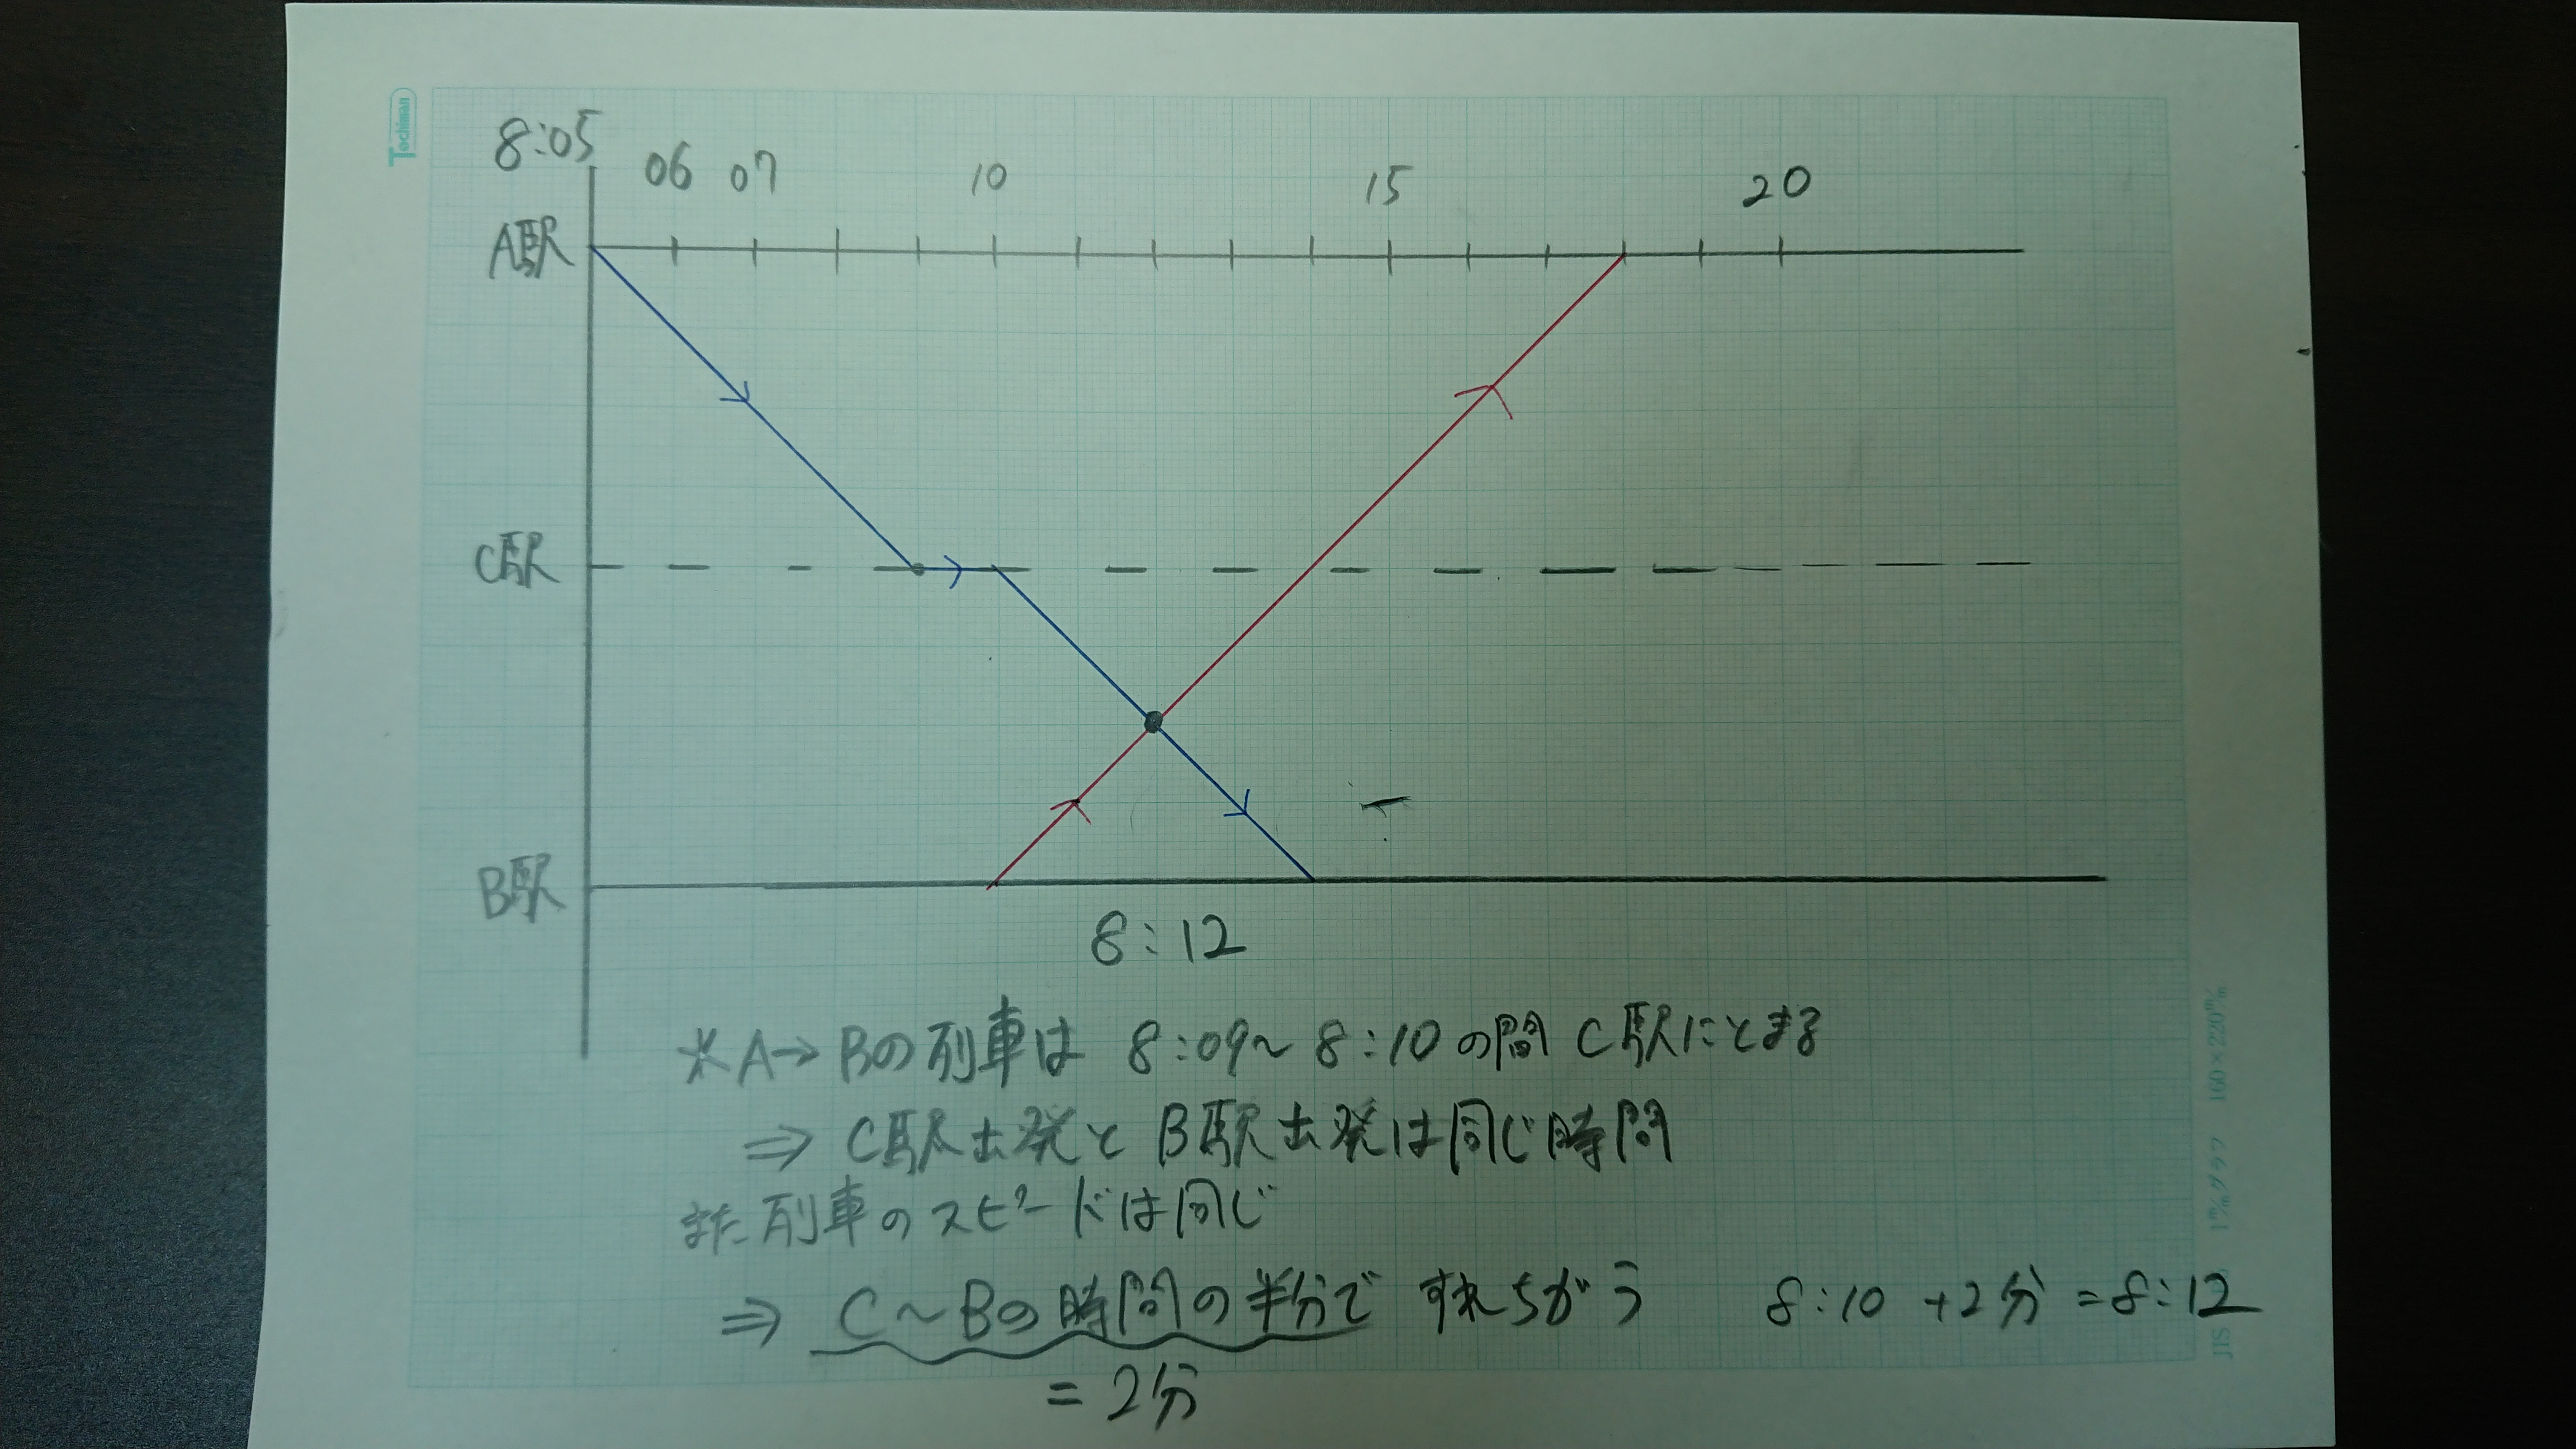
\includegraphics[height=6cm]{0421_01_1.jpg}
			\caption{解答}
			\label{jpg:0421_01_1}
		\end{figure}

	\end{frame}

	\begin{frame}{解答3-2}
		\begin{figure}[htbp]
			\centering
			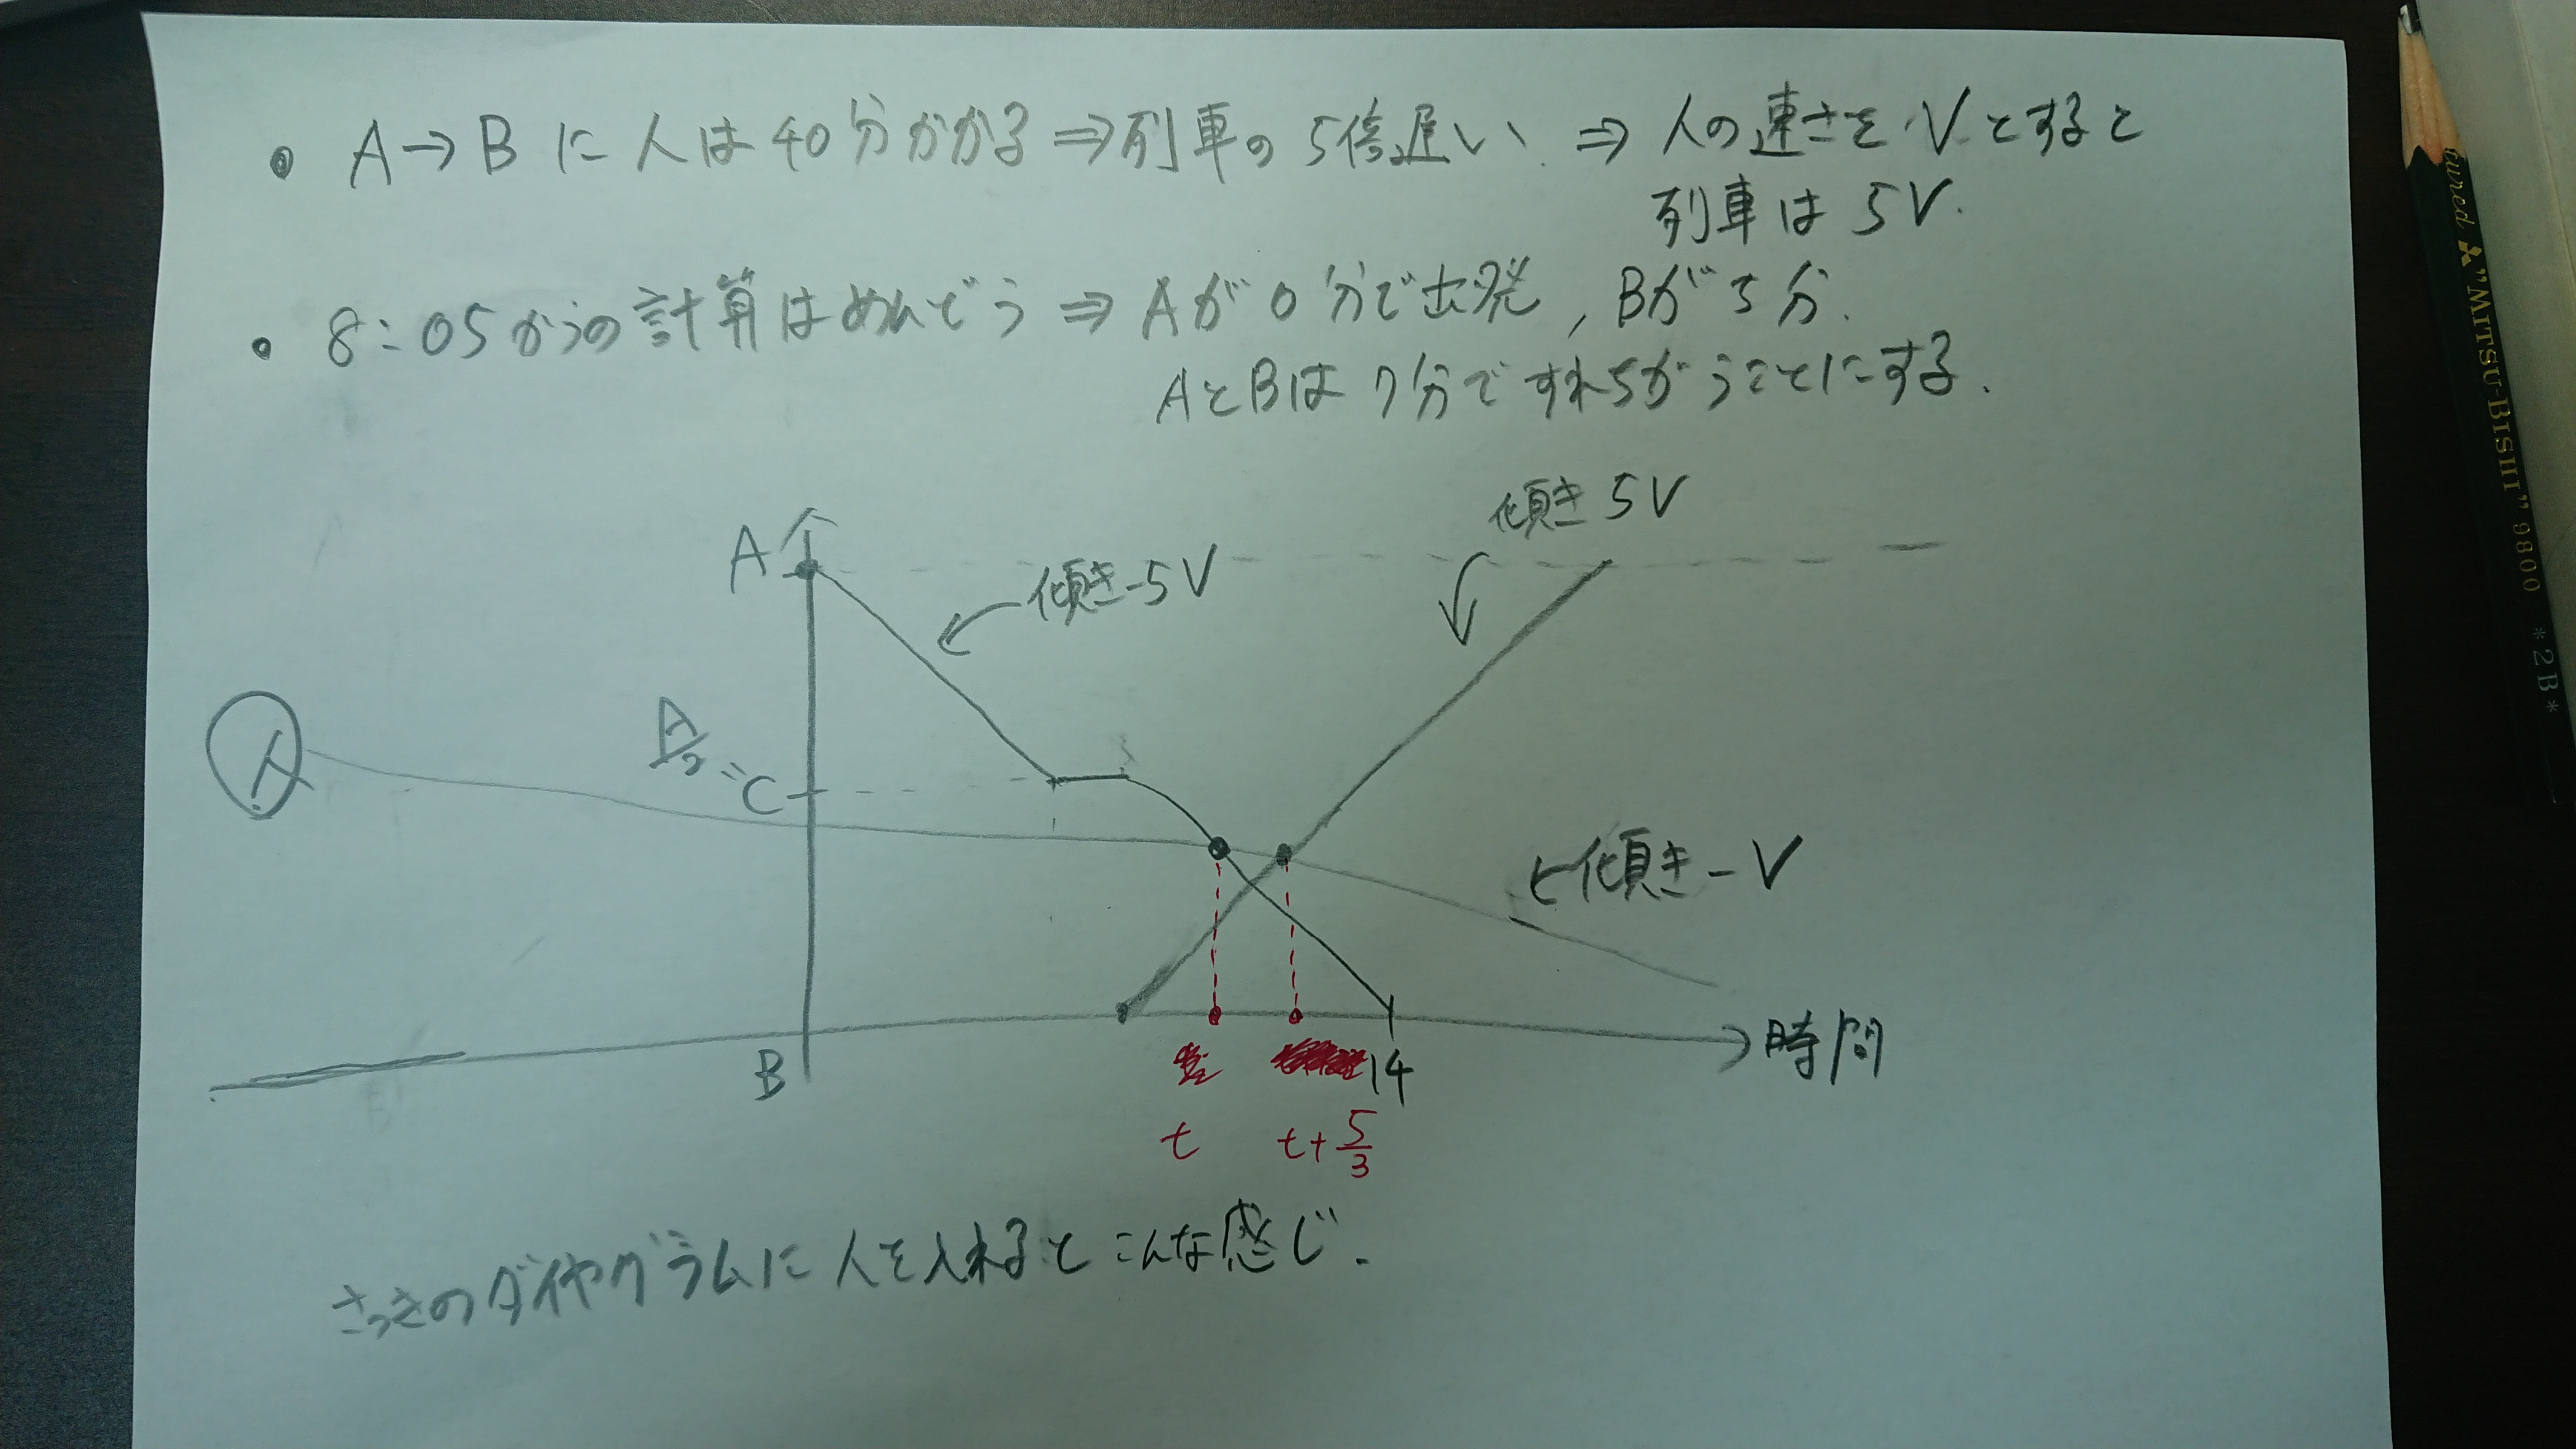
\includegraphics[height=6cm]{0421_01_2.jpg}
			\caption{解答}
			\label{jpg:0421_01_2}
		\end{figure}
	\end{frame}

	\begin{frame}{解答3-3}
		\begin{figure}[htbp]
			\centering
			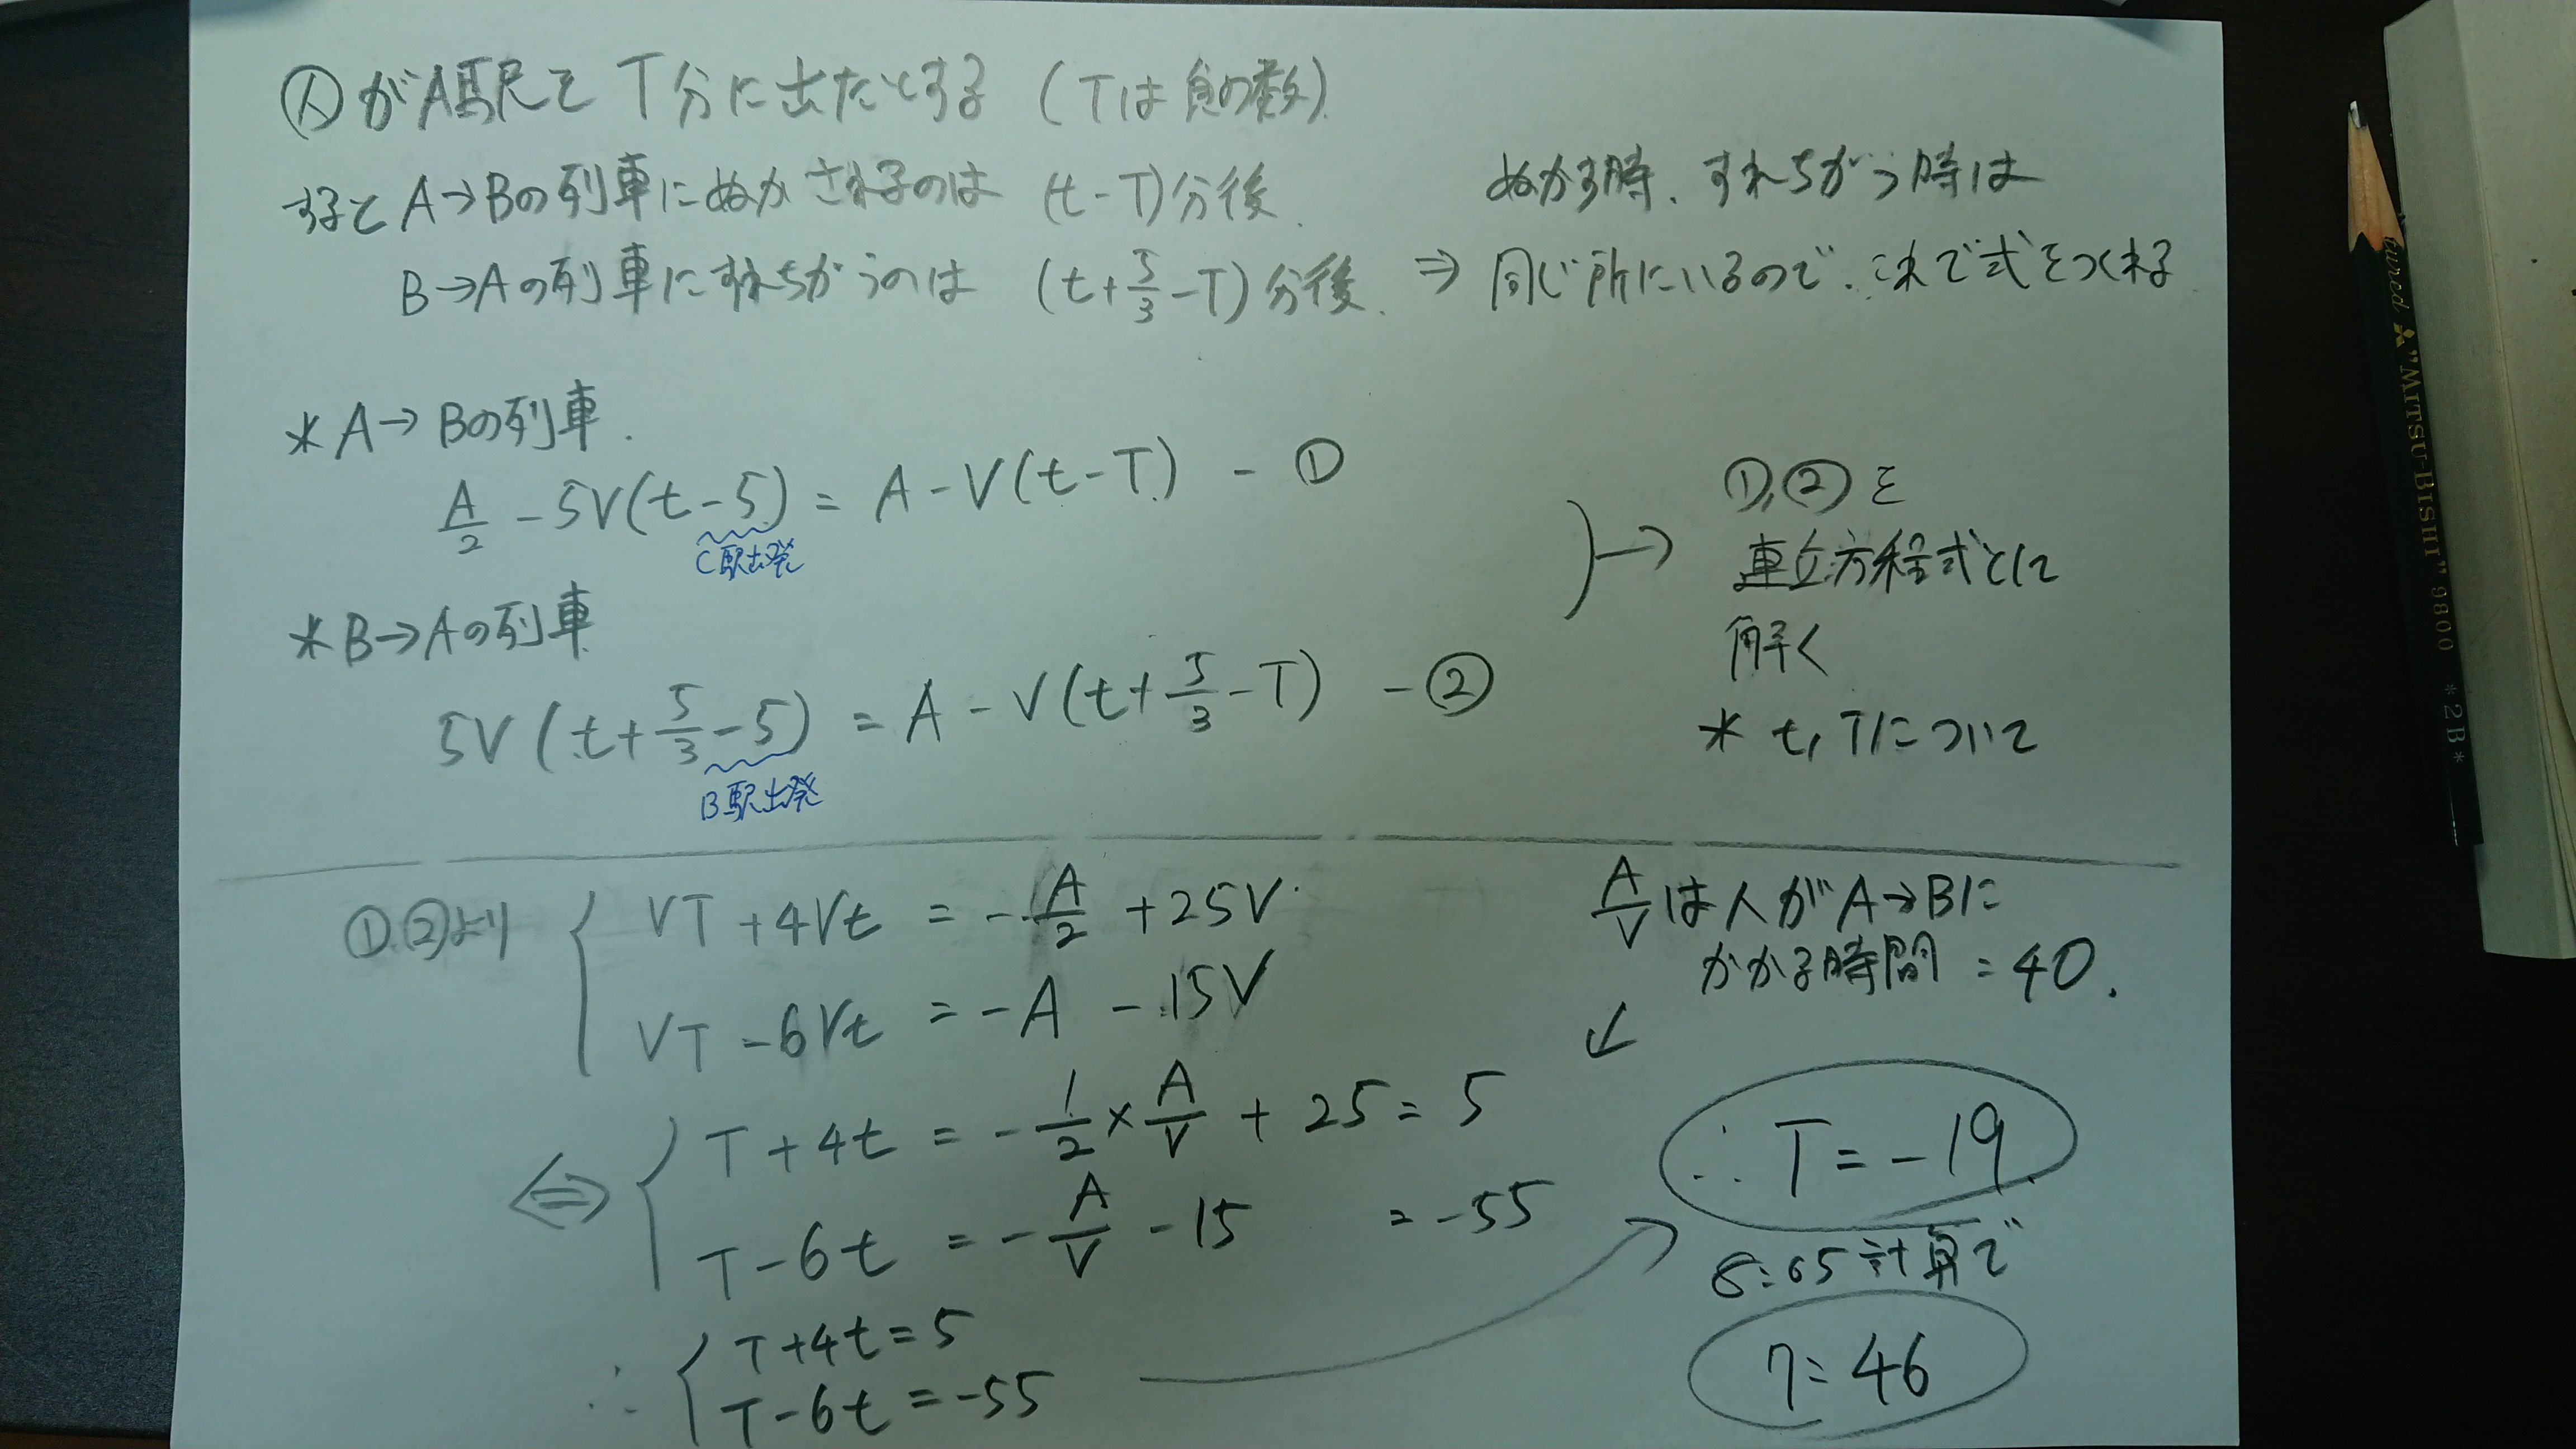
\includegraphics[height=6cm]{0421_01_3.jpg}
			\caption{解答}
			\label{jpg:0421_01_3}
		\end{figure}
	\end{frame}



	\begin{frame}{問題4}
		\begin{figure}[htbp]
			\centering
			\includegraphics[width=\textwidth]{0421_02.jpg}
			\caption{問題}
			\label{jpg:0421_02}
		\end{figure}


	\end{frame}

	\begin{frame}{解答4}
		\begin{figure}[htbp]
			\centering
			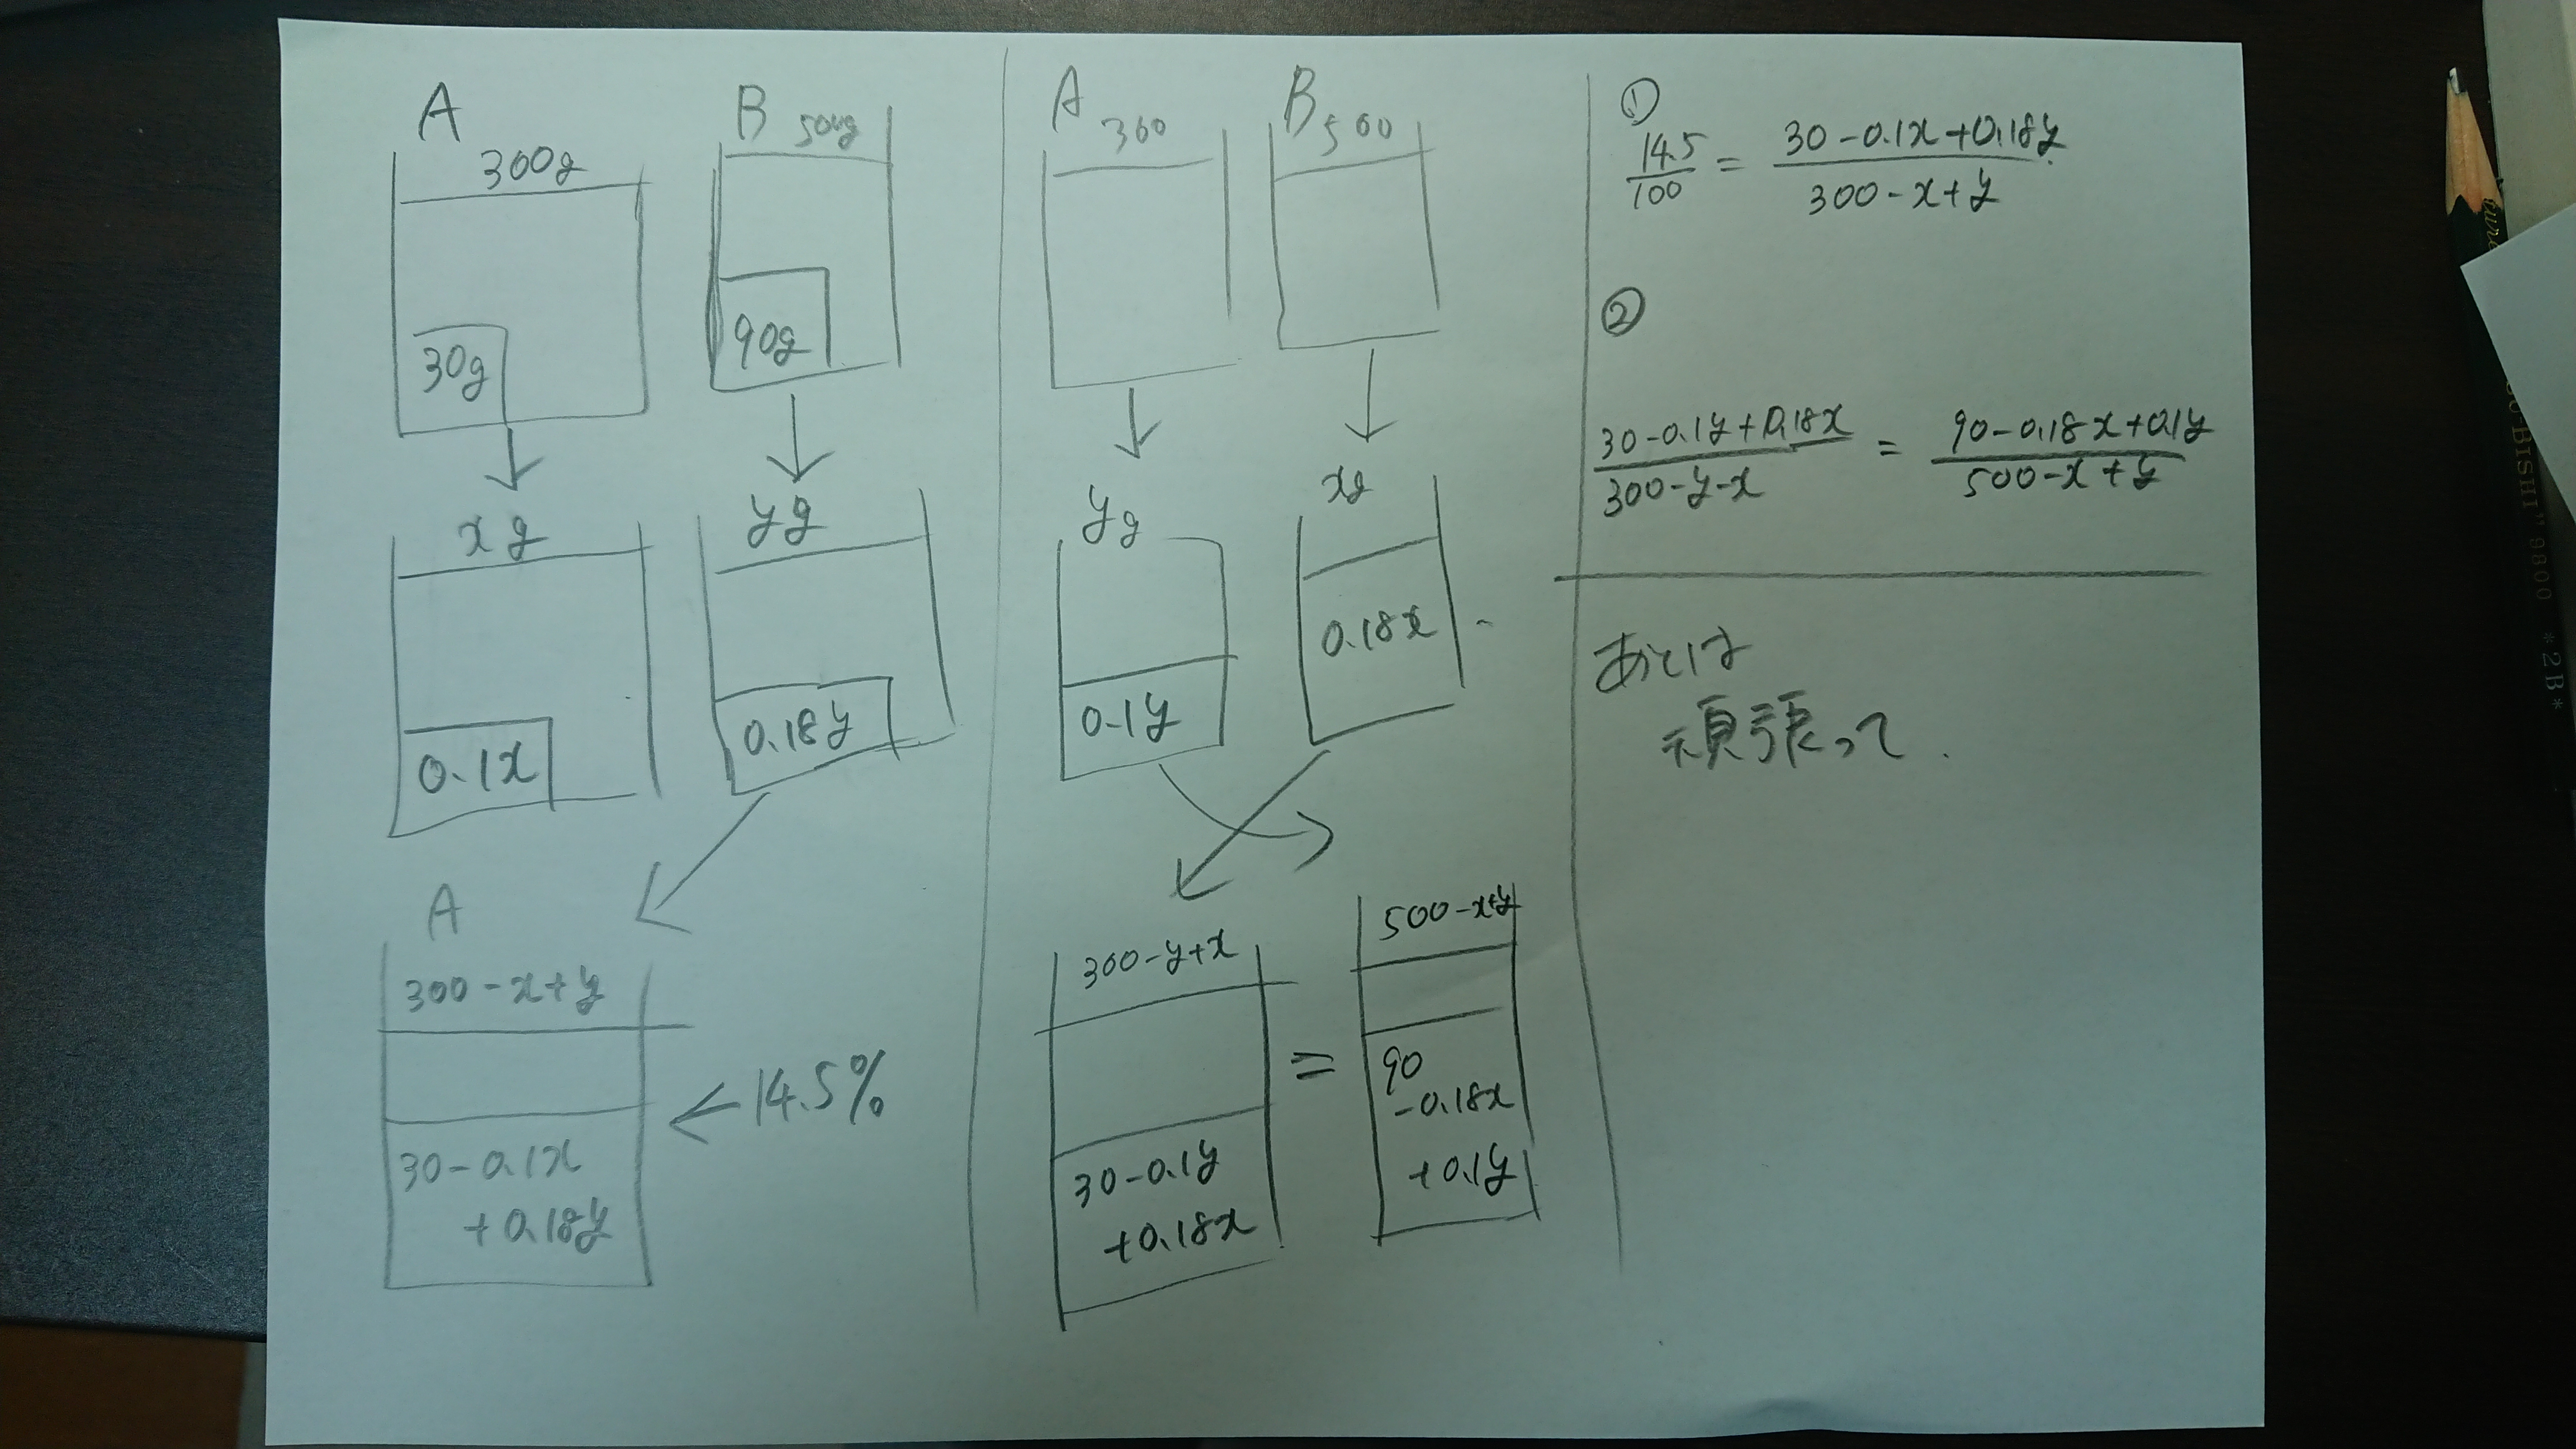
\includegraphics[height=6cm]{0421_02_1.jpg}
			\caption{解答}
			\label{jpg:0421_02_1}
		\end{figure}
	\end{frame}

	\begin{frame}{所感}
		前回の資料にもある通り,一度に扱う問題の数は少しだけです.
		問題を送る数を考えてください.
		% また,
		% 僕の力を測ろうとするような問題には以降解答しません.

		次回は未定ですが,扱う問題は1,2題までです.
		% 調子に乗って問題をたくさん送りつけてくる場合は
		% 面倒なので,勉強会やめます.
	\end{frame}

\end{document}

